\documentclass[conference,10pt]{IEEEtran}
%\documentclass[conference,draft,onecolumn]{IEEEtran}
% useful packages, copy and paste from diff sources

\usepackage[english]{babel}
\usepackage[T1]{fontenc}
\usepackage{cite,url,color} % Citation numbers being automatically sorted and properly "compressed/ranged".
\usepackage{graphics,amsfonts}
\usepackage{epstopdf}
\usepackage[pdftex]{graphicx}
\usepackage[cmex10]{amsmath}
%\DeclareMathOperator*{\argmax}{arg\,max}
%\DeclareMathOperator*{\argmin}{arg\,min}
% Also, note that the amsmath package sets \interdisplaylinepenalty to 10000
% thus preventing page breaks from occurring within multiline equations. Use:
\interdisplaylinepenalty=2500
% after loading amsmath to restore such page breaks as IEEEtran.cls normally does.
\usepackage[utf8]{inputenc}
% Useful for displaying quotations
%\usepackage{csquotes}
% Compact lists
%\let\labelindent\relax
\usepackage{enumitem}

%tikz figures
\usepackage{tikz}
\usetikzlibrary{automata,positioning,chains,shapes,arrows}
\usepackage{pgfplots}
\usetikzlibrary{plotmarks}
\newlength\fheight
\newlength\fwidth
\pgfplotsset{compat=newest}
\pgfplotsset{plot coordinates/math parser=false}

\usepackage{algorithm}
\usepackage{algorithmic}
%\usepackage{algpseudocode}

\usepackage{array}
% http://www.ctan.org/tex-archive/macros/latex/required/tools/
%\usepackage{mdwmath}
%\usepackage{mdwtab}
%mdwtab.sty	-- A complete ground-up rewrite of LaTeX's `tabular' and  `array' environments.  Has lots of advantages over
%		   the standard version, and over the version in `array.sty'.
% *** SUBFIGURE PACKAGES ***
%\usepackage[tight,footnotesize]{subfigure}
\usepackage{subfig}

\usepackage[top=1.5cm, bottom=2cm, right=1.6cm,left=1.6cm]{geometry}
\usepackage{indentfirst}

\usepackage{times}
% make sections titles smaller to save space
%\usepackage{sectsty}
%\sectionfont{\large}
% enable the use of 'compactitem', a smaller 'itemize'
%\usepackage{paralist}

% MP
% to split equations using dmath env
\usepackage{breqn}
% nice rules in tables
\usepackage{booktabs}

%\setlength\parindent{0pt}
\linespread{1}

% MC
\newcommand{\MC}[1]{\textit{\color{red}MC says: #1}}
\newcommand{\AZ}[1]{\textit{\color{blue}AZ says: #1}}
\newcommand{\MP}[1]{\textit{\color{green}MP says: #1}}

\usepackage{placeins}

%%%%%%%%%%%%%%%%%%%%%%%%%%%%%%%%%%%%%%%%%%
\begin{document}
%%%%%%%%%%%%%%%%%%%%%%%%%%%%%%%%%%%%%%%%%%
\title{A Greedy Approach for Proactive	Caching	in	Mobile	Scenarios	with 5G mmWave	Communications}

\author{\IEEEauthorblockN{Ludovico Frizziero,
				  		Alberto Suman,
			  	  		Anthony Dell'Eva}
\IEEEauthorblockA{Department of Information Engineering, University of Padova -- Via Gradenigo, 6/b, 35131 Padova, Italy\\Email: {\tt\{ludovico.frizziero,alberto.suman,anthony.delleva\}@studenti.unipd.it}
}}

\maketitle

%% enable page numbering %%
%\thispagestyle{plain}
%\pagestyle{plain}
%%%%%%%%%%%%%%%%%%%%%%%%%%%

\begin{abstract}
Fifth generation networks (5G) are going to revolutionize communications in the next years, but, nowadays, there are still several challenges to overcome. Due to small cells size, mobility users experience long handover delays, and the quality of specific applications, e.g. video streaming, is degradated. Avoidance of unintended latencies is provided by proactively loading the file content from the remote server to the cache of the base stations which the user will connect to. Our heuristic proactive caching algorithm obtains optimal QoS for 4K video streaming in a highway scenario.\\

\textit{Index Terms}---proactive caching, 5G, mobile video streaming, millimeter wave channel.
\end{abstract}




%%%%%%%%%%%%%%%%%%%%%%%%%%%%%%%%%%%%%%%%%
\section{Introduction}\label{sec:intro}
%%%%%%%%%%%%%%%%%%%%%%%%%%%%%%%%%%%%%%%%%
The very rapid dissemination of mobile devices in the last years and the resulting growth of multimedia traffic have created new challenges for internet providers. Next generation technologies for mobile communications (5G) can face the overwhelming demand thanks to higher data rates, lower latencies and strong reliability. Nowadays, the lack of a standard for 5G is basically due to a poor knowledge of the millimeter wave (mmWave) channel, with operating frequencies from  20 GHz up to even 300 GHz. The proactive caching problem, addressed in this paper, is caused by the propagation behaviour of signals transmitted over this spectrum and, in particular:
\begin{itemize}
\item the reduced diffraction properties make it difficult for these signals to cross blockages and the channel keeps an on/off evolution depending on the presence or absence of LoS (Line-of-Sight). Furthermore, the free-space pathloss between transmit and receive antennas grows with the square of the carrier frequency.  In a real environment, for these reasons, network cells can only have ranges under 100 meters (picocells) or ranges of a few meters (Wi-fi like range, femtocells);
\item mmWave beams are highly directional, making antennas and associated gains very susceptible to misaligned beams [1-3].
\end{itemize}
Globally, according to the 09/2017 Cisco Visual Networking Index, IP video traffic will be 82\% of all consumer Internet traffic by 2021. High quality video streaming services have to deal with important challenges in 5G networks, given the channel peculiarities described above. In a mobility scenario, like the one proposed in our simulation, users have frequent handovers between cells and a proactive caching system is crucial to cut delays and transmission overheads caused by the reconstruction of the path from the mobile device to the remote server. The system shall be able to optimize the video content allocation to the storages of the base stations (BSs) deployed along the user way, removing the added latency due to new connections and the video frozenness that has a significant impact on the streaming quality.

We propose a greedy approach to determine a suboptimal solution for proactive caching problem, attaining  high quality of service (QoS) for 4K-60fps video streaming. We considered a highway scenario, where vehicles move with velocities from 70 to 130 kmph. The amount of memory that a BS can allocate depends on the free space still available and on the numbers of users connected to it, while the choice of the effectively allocated BS is made by a greedy algorithm that determines a pattern which is able to evenly cover the stretch of road considered, given the initial parameters. Our approach outperforms a random allocation of BSs storages and a random selection of BSs along the highway sector considered. The results can be extended and exploited also in all the cases where the path is predetermined (e.g., autonomous vehicles).

The remainder of the paper is organized as follows. Section II is an overview of the related works addressing the problem of proactive caching and its optimization. Section III introduces the system model and the choices we made for our Matlab simulation, while Section IV shows the proposed solution. Performance results and conclusions are, respectively, in Section V and VI.
%%%%%%%%%%%%%%%%%%%%%%%%%%%%%%%%%%%%%%%%%%%%
\section{Related Work}\label{sec:sota}
%%%%%%%%%%%%%%%%%%%%%%%%%%%%%%%%%%%%%%%%%%%%
Recently, with the advent of 5G technologies, the problem of proactive caching is becoming more and more important, not only for its contribute in providing high quality streaming services.

In [9], Quiao et al. propose a system where the cache management problem is formulated as a Markov decision process. A cell-by-cell decomposition is then used to solve the dynamic programming problem with reduced computational complexity. Here, unlike our work, the solution follows a rigorous mathematical theory and not an heuristic approach.

In [10] is proposed a procedure that exploit the social structure of the network by predicting the set of influential users to cache strategic contents. BSs build a model solving a minimization problem with  a so called popularity matrix, where row represents users and columns file preferences/ratings, and the already available informations regarding users' preferences. After obtaining the matrix, the proactive caching decision can be made by storing the most popular files greedily until no storage remains.

Ahlehagh [11] addresses the problem of video caching in radio access network. The proposed caching architecture consists of a very large BSs micro-caches, each one being able to store only 1000s of videos, unlike Internet CDNs that can store millions of videos in a relatively few large sized caches. Obviously, the hit rate may not be high: two caching policies are proposed based on preferences profiles of users in a cell and their associated video request probabilities.

Mishra et al. [12] solve the proactive caching problem using a novel and efficient data structure (neighbor graphs), that captures the mobility topology of a wireless network and exploits it for pre-caching the station context, ensuring that it always remains one hop ahead. Neighbor graphs can reduce layer 2 latency handoff by an order of magnitude.



%%%%%%%%%%%%%%%%%%%%%%%%%%%%%%%%%%%%%%
\section{System Model}\label{sec:symo}
%%%%%%%%%%%%%%%%%%%%%%%%%%%%%%%%%%%%%%

\begin{figure*}
	\centering
	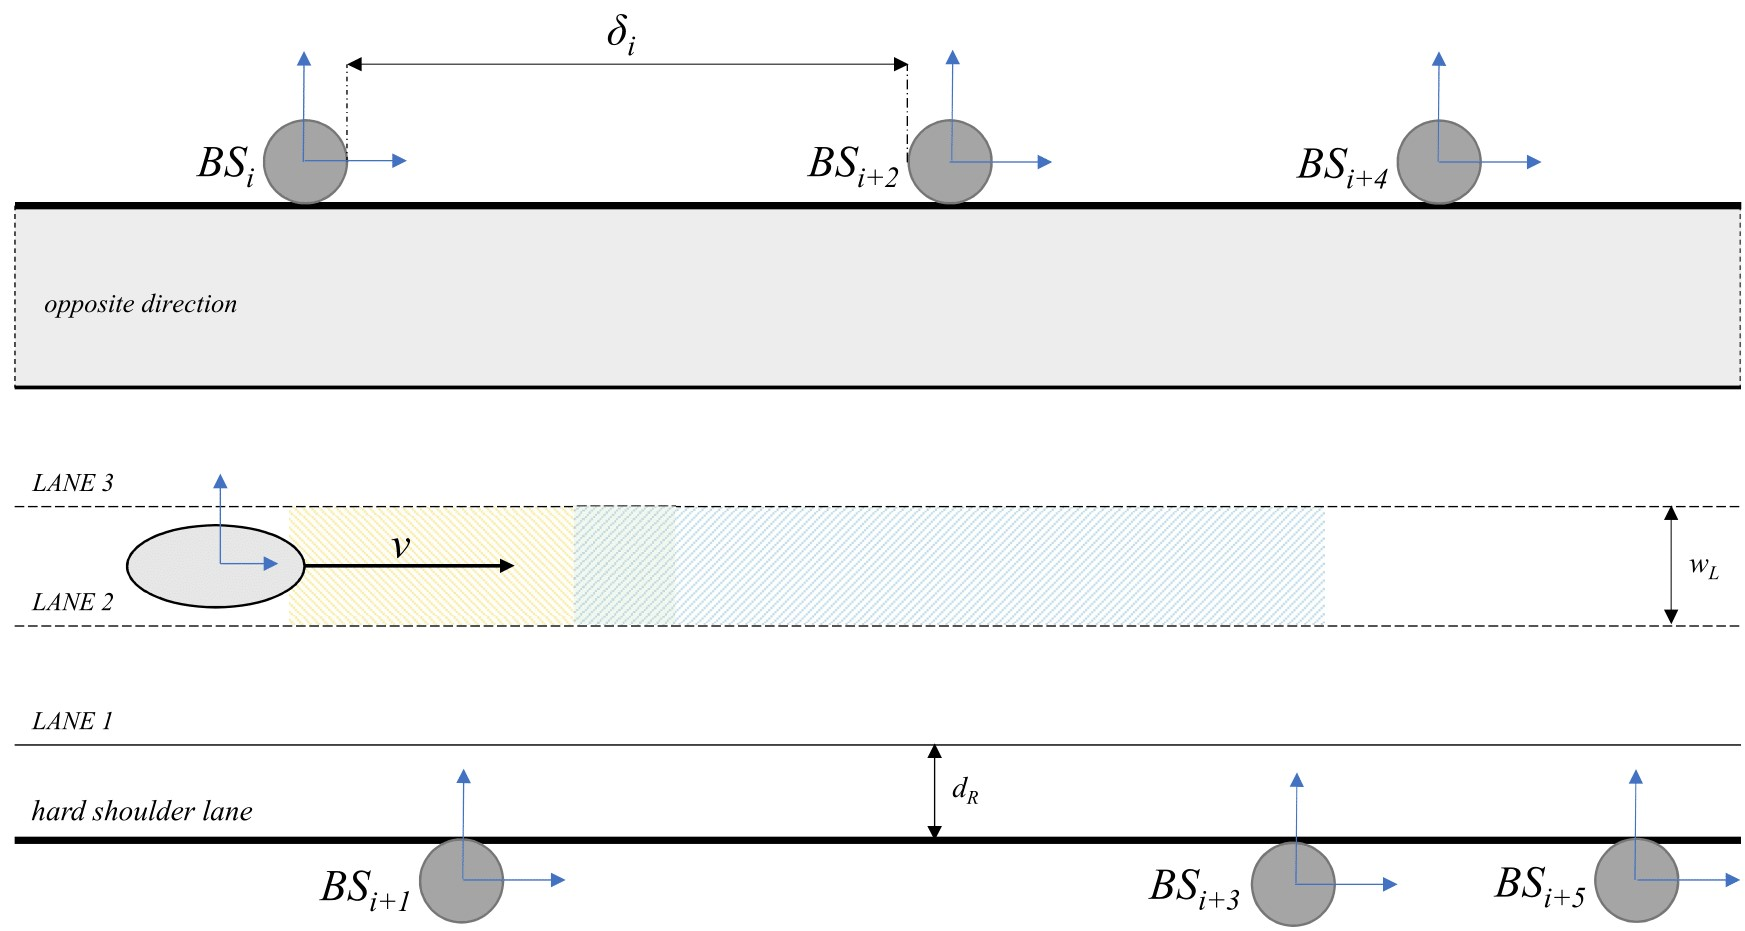
\includegraphics[width=0.9\textwidth]{highway1.jpg}
	\caption{representation of the highway sector. The yellow and the blue areas denote the support zones of the (i+1)-th and of the (i+2)-th BSs respectively.}
	\label{fig:highway_sector}
\end{figure*}

This section describes the model used for the simulation. In particular we discuss about the highway scenario, the wireless network architecture and, finally, the proposed solution for the proactive caching problem.

\subsection{Highway Scenario}
In the simulation we utilize a 1 km straight sector of the highway with three lanes for each direction. The sector is represented in Fig. \ref{fig:highway_sector}. For every iteration we consider a single user entering the road in one of the lane which is randomically chosen. The user's expected speed is $v_0$, while the instanteneous speed varies every $dt = 0.1\, s$ such as
\begin{equation}
	\label{eq:speed}
	v = v_0+a\cdot dt \quad [m\!/\!s]
\end{equation}
where $a$ indicates the acceleration, which is chosen randomically each second between $a_{min}=-10\,m\!/\!s^2$ and $a_{max}=10\,m\!/\!s^2$. The speed the user can have is also bounded to be in the interval $v \in v_0 \pm v_0 \cdot 10\%$. This is a somewhat hard constraint, although not completely unrealistic.

\subsection{Network Architecture}
For this paper we used a 5G wireless network architecture to provide high data rate in most coverage areas. The parameters of the channel are given in Tab.\ref{tab:params}. Base stations (BS) are deployed in each side of the road according to a Poisson distribution with mean $\lambda_{BS}$, hence the total expected amount of base station per sector is $2\lambda_{BS}$. The distance from the i-th BS to the next one within the same row is given as
\begin{equation}
	\label{eq:distance}
	\delta_i = \frac{1000}{\lambda_{BS}}+u_i \quad [m]
\end{equation}
where $u_i$ is generated by an uniform distribution in the interval $[-500\cdot\lambda_{BS}^{-1},500\cdot\lambda_{BS}^{-1}]$. This means that usually BSs tend to be uniformly spaced apart, but it can happen that some BS may end up being very close one another.  

The number of users for each BS is renewed every second with a value given by a poisson distribution with parameter $\lambda_{U\!E}$. Thus the available bandwidth for the user at the i-th BS is
\begin{equation}
	\label{bandwidth}
	BW_{U\!E,i} = \frac{BW}{m_i}
\end{equation}
where $m_i$ indicates the number of users at the i-th BS.
Every $dt$ the rate from the i-th BS which the user equipment (UE) is connected to to the UE itself is calculated as
\begin{equation}
	\label{eq:rate}
	r_i = BW_{U\!E,i}\cdot\log_2(1+SINR) \	
\end{equation}
where in the SINR computation we used the path-loss model given by
\begin{equation}
	(PL_i)_{dB} = 32.4+20\log_{10}(d)_m+20\log_{10}(f_c)_{M\!H\!z}+\Psi
\end{equation}
with $\Psi\sim \mathcal{N}(0,6)$ taking into account the shadowing. We consider also an outage threshold, below which it is set $r_i = 0$.

Furthermore, the BSs and the UE are provided with electronically steerable directional antennas. BSs take advantage of MIMO techniques, as spatial multiplexing and spatial beamforming to improve, respectively, rate and channel gain (we used 16 antennas for each BS and 4 antennas for the UE). The latter is computed from the Channel State Information matrix, which is completely updated every $3\cdot dt$ seconds, while signal scattering due to subpaths is recomputed every $dt$.

Finally, the BSs' network drives the handover in an optimal way: the users is forced to connect only to those BS that have memory available for him, in an order induced by the UE's travel direction, and only when it is proper to due so, that is only when the UE is about to enter the support region of the next BS. The concept of support region is introduced later in [eq. \ref{eq:support-region}].

\begin{center}
	\begin{table}
		\caption{Parameters of the road and of the channel.}
		\label{tab:params}
		\begin{center}
			\begin{tabular}{lcc}
				\toprule
				Parameter	&	Symbol	&	Value	\\
				\midrule
				hard shoulder width				&	$d_R$		&	2.5 m	\\
				lane width						&	$w_L$		&	3.75 m	\\
				carrier frequency				&	$f_L$		&	28 GHz	\\
				line-of-sight coefficient		&	$\alpha_L$	&	2		\\
				non-line-of-sight coefficient	&	$\alpha_N$	&	2.92	\\
				transmitting power				&	$P_{tx}$	&	27 dBm	\\
				bandwidth						&	$BW$		&	1 GHz   \\
				\bottomrule
			\end{tabular}
		\end{center}
	\end{table}
\end{center}

\subsection{User Behavior}

The user needs to download a huge file $F$ (such that it can't be downloaded entirely within the premises of the highway sector we consider) from the internet. We consider the file to be compressed, such that to require a minimum rate $\mu_{U\!E} \in [0.06, 0.15]$ Gbits/s in order to be played back/consumed correctly by the user. The user also has at its disposal a buffer $\Omega$ that allows to store 15 seconds of content, that is
\begin{equation}
\Omega = 15 \cdot \mu_{U\!E} \quad [bits]
\end{equation}

 As soon as the UE is connected to a BS that has memory allocated for him, it starts downloading the available chunk of file with the rate $r_i$ provided by the connection, and to store it in its buffer. There is no flow control, therefore it may happen some portion of the file are lost due to buffer overflow. Lost data are not currently retransmitted. We also consider the download process as a stream of bits rather than packets, since channel errors are not considered. This allows to evaluate for maximum and ideal performances of our system.
 
\section{Proposed Solution}
 
This section describes the problem we want to solve, then it provides the solution, correlated with pseudocode for the solver for the related optimization problem.

\subsection{Problem Statement}

We want to achieve as uniform as possible performances of our system across all range of speeds the user can have, regardless of the underlying BS density and memory availability in each of them, while keeping the communication overhead among the central controller (CC), required for coordination, and all the BSs as low as possible. 

The overhead is reduced thanks to two main assumptions: 
\begin{itemize}
	\item each highway sector is thought as independent from the others, therefore each of them has its own local controller;
	\item every BS manages the memory regardless of the others.
\end{itemize}
When a UE is going to enter the sector, the relative CC is notified. It then computes an optimal size of memory to allocate to the eventually selected BS based on the actual mean speed of the UE and the density of base stations on the sector, as
\begin{equation}
m = \alpha_{v_0, \lambda_{B\!S}} \cdot \tau \cdot \mu_{U\!E} \quad [bits]
\end{equation}

where $\tau = (1000/\lambda_{B\!S})/v_0$ is the mean connection time to a BS the UE can experience on the sector, and $\alpha_{v_0, \lambda_{B\!S}} > 0$ is a scale factor used to tune performances. In particular it is strictly tied to the optimal number of base stations the CC ends up allocating along the highway. Every BS within the premises of the CC must then only report if it has such memory space available or not. This eases communication overhead because the CC doesn't have to keep a record of the memory state for each base station constantly updated.

Now that the CC knows all the candidate BSs, an optimal number among them must be chosen to receive a chunk of the file requested by the UE. This is possible by defining the concept of support of the i-th BS as
\begin{equation}
\label{eq:support-region}
S_i = g_i(m)\frac{v_0}{\mu_{U\!E}} \quad [m]
\end{equation}

that is, for how many meters the UE can travel only relying on its buffer after he downloaded all the memory $g_i(m)$ the i-th BS had allocated for him, before experiencing file playback freezing. This measure, due to $v_0$, is of course, only in expectation. The support is also thought as centered on its relative BS, but this is not important as long as its starting point is decided with a common rule for each BS. Instead, $g(\mathbf{m})|_i \doteq g_i(m)$, where $\mathbf{m} \in \{0, m\}^N$ is the vector containing the memory report for each BS in the sector, is a function introduced later that determines how much memory the CC eventually allocates to the i-th BS. The optimal number of BSs to choose is then found as $\mathbf{S}^T\mathbf{x} \approx 1000$, where $\mathbf{x} \in \{0,1\}^N$ is the (binary) choice vector outputted by the CC, and  $\mathbf{S} \in \mathbb{R}_+^N$ is the vector that contains the support for each BS.

Finally, it is also necessary to evenly distribute the chosen BSs along the sector, to assure buffer overflows are minimized and playback freezing is avoided. To this avail the final optimization problem has a cost term that depends on a vector $\mathbf{d} \in \mathbb{R}_+^N$ which captures the relevant distances among chosen base stations, that is, given $\mathbf{x} \in \{0,1\}^N$, each component is defined as

\begin{figure}[t]
	\centering
	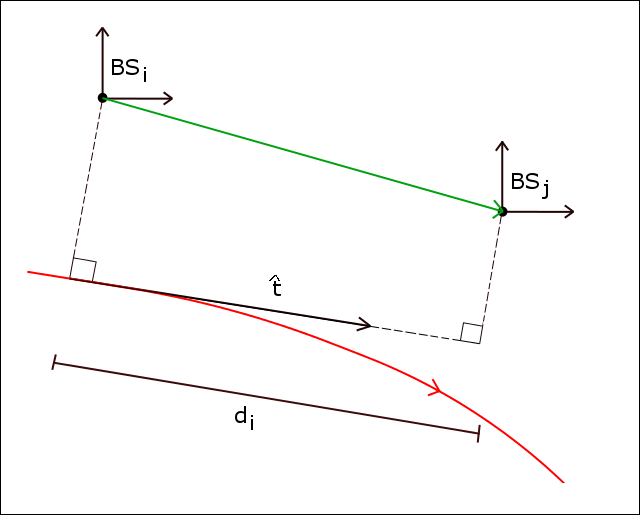
\includegraphics[width=9cm]{BS_distance.png}
	\caption{representation of minimum distances from [eq. \ref{eq:dists}] }
	\label{fig:min_dists}
\end{figure}

\begin{equation}
\label{eq:dists}
d_i = \min_{j \textrm{ s.t. }x_j = 1} |<pos_w(BS_i) - pos_w(BS_j), \hat{t}_{w, i}>|
\end{equation} 

Here $\hat{t}_{w, i}$ is the unitary norm tangent to the travel direction (predicted along the sector) of the UE in world coordinates, evaluated on the perpendicular of the i-th BS, while $pos_w(BS_i)$ is the position of the i-th BS in world coordinates. A representation is visible in Fig.\ref{fig:min_dists}.

\subsection{Optimization Problem}

The proposed optimization problem therefore is

\begin{center}
	\begin{tabular}[h]{|c|}
		
		\hline
		OPTIMIZATION PROBLEM \\
		\hline
		\makebox[8.6cm]{
			$			
			\begin{array}{l l l l l l}
				\null \\
				\mathbf{x} \in \underset{\mathbf{x} \in \{0,1\}^N}{argmax} {\textrm{ } \sum_i{g_i(m)x_ie^{-\frac{(\mathbf{S}^T\mathbf{x} - 1000)^2}{2}}} - \lambda\left(\frac{\mathbf{d}^T\mathbf{x}}{2} - 1000\right)^2} \\[3ex]
				\textrm{such that:}\\[0.5ex]	
				\sum_i{g_i(m)x_i} \le F\\[0.5ex]		
				0  < g_i(m) \le min(m, \Omega) \textrm{ } \forall i \textrm{ s.t. } x_i  = 1 \textrm{,   0 otherwise}
				\null \\[2ex]
			\end{array}
			$
		}\\
		\hline
	\end{tabular}
\end{center}

where $\lambda > 0$ is a tradeoff parameter between memory allocation and its even distribution along the sector. The function $g(\cdot)$ allows for some flexibility from the CC side in distributing the memory, such that in some BS it may end up being less than what originally requested if needed for any reason. This is especially useful to avoid having overlapping supports between chosen base stations, because this may cause buffer overflow at the user side. In particular a useful expression for $g(\cdot)$ that minimizes such overlaps, given the almost uniform BSs' deployment assumed in this paper, is 

\begin{equation}
g_i(m) = min\left(\frac{1000\mu_{U\!E}}{v_0 ||\mathbf{x}||_0}, m\right)
\end{equation} 

because this makes the support $S_i$ become exactly the expected distance among BSs after having observed which one has been chosen, that is

\begin{equation}
S_i = \mathbb{E}{[\delta_{i, j}| \mathbf{x}]} =  \frac{1000}{\textrm{ }||\mathbf{x}||_0}
\end{equation} 

The expression $||\cdot||_0$ is the zero norm of a binary vector. The discussion made so far presents the solution that best maximizes our optimization problem given the geometric assumption it relies on. It is nonetheless possible to lessen the uniform constraint over $m$, or over $g(\cdot)$, but the solution becomes suboptimal. 

Finally we provide the pseudocode that solves the optimization problem in [Alg. \ref{alg:solver}], that runs approximately in $O(N^4)$ due to the update on $\mathbf{d}$. At first it solves the optimization problem by considering the requested amount $m$ for each BS. This way an optimal number of stations is selected, then it applies $g(\cdot)$ in order to minimizes support regions overlapping, while also maximizing the exponential to 1 as a (desired) byproduct.

\begin{algorithm}
	\caption{pseudocode to solve the optimization problem}
	\label{alg:solver}
	\begin{algorithmic}
		\STATE \textbf{Input:} $\mathbf{m} \in \{0, m\}^N, \textrm{ } F$, positions of each BS with respect to the world
		\STATE \textbf{Output:} $\mathbf{x} \in \{0, 1\}^N, \textrm{ } g(\mathbf{m}) \in \{0, g_i(m)\}^N$
		\STATE \null
			\STATE $\mathbf{x} \leftarrow \mathbf{0}$, $x_i \leftarrow 1$ for a random $i$
			\STATE $\mathbf{S} \leftarrow (\mathbf{m}v_0)/\mu_{U\!E}$
			\WHILE {$\mathbf{S}^T\mathbf{x} < 1000$ \OR $\mathbf{m}^T\mathbf{x} \le F$ }
				\STATE best_i $\leftarrow$ invalid index, best_k $\leftarrow -\infty$ 
				\FOR{$j \in \{1..N\}/\{i : x_i = 1\}$}
					\STATE $\mathbf{y} \leftarrow \mathbf{x}$, $y_j \leftarrow 1$
					\STATE $\mathbf{d} \leftarrow$ update distances as in [eq. \ref{eq:dists}] with reference to    	$\mathbf{y}$
					\STATE $k \leftarrow \mathbf{m}^T\mathbf{y} - \lambda\left(\frac{\mathbf{d}^T\mathbf{y}}{2} - 1000\right)^2$
					\IF{k > best_k}
						\STATE best_k $\leftarrow k$, best_i  $\leftarrow j$
					\ENDIF
				\ENDFOR 
				
				\IF{best_i \NOT invalid}
					\STATE $x_{best\_i} \leftarrow 1$
				\ELSE
					\STATE CONSTRAINTS NOT MET
				\ENDIF
			\ENDWHILE
			\STATE $g(\mathbf{m}) \leftarrow \mathbf{0}$
			\FORALL {i = \{1...N\}}
				\STATE 	$g_i(m)\leftarrow \frac{1000\mu_{U\!E}}{v_0||\mathbf{x}||_0}$ if $x_i=1$, 0 otherwise
 			\ENDFOR
			\RETURN $\mathbf{x}$, $g(\mathbf{m})$
	\end{algorithmic}
\end{algorithm}


\begin{figure*}[t]
	\centering
	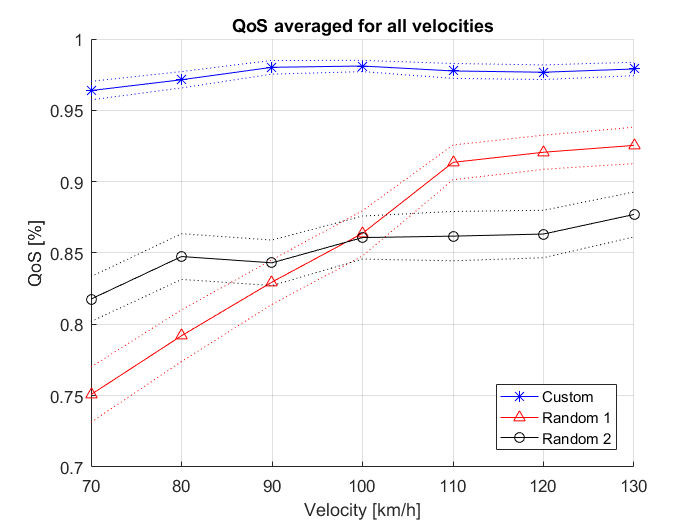
\includegraphics[width=9cm]{QoS.png} 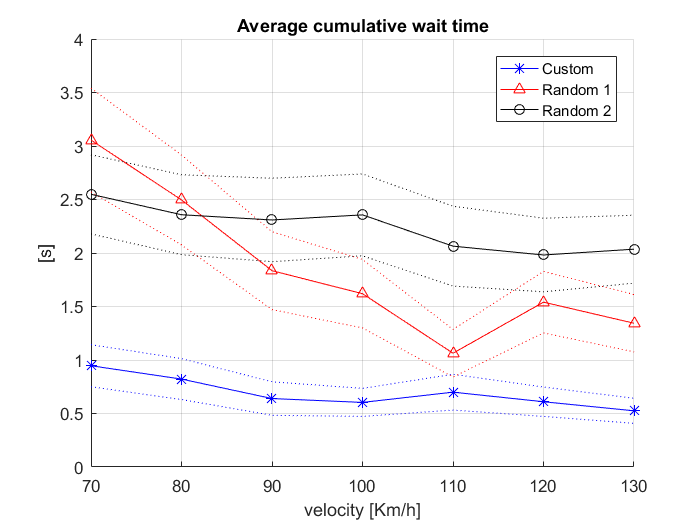
\includegraphics[width=9cm]{UE_wait_time.png}
	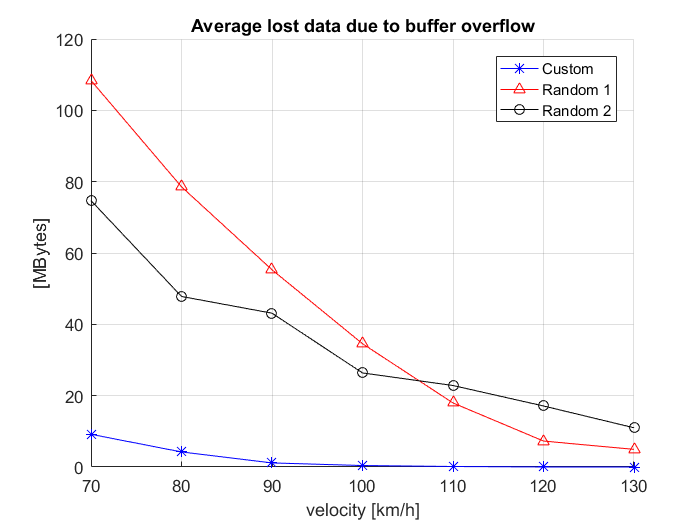
\includegraphics[width=9cm]{UE_buffer_overflow.png} 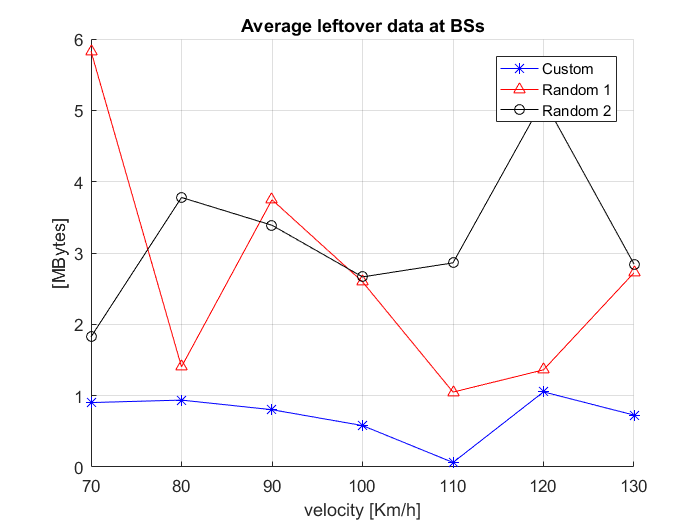
\includegraphics[width=9cm]{BS_leftover_data.png}
	\caption{Statistics for a sector with density of 14 BS. Confidence Intervals at 95\% are shown were relevant.}
	\label{fig:7BS_all_stats}
\end{figure*}

%%%%%%%%%%%%%%%%%%%%%%%%%%%%%%%%%%%%%%%%%%%%%%%
\section{Results}\label{sec:res}
%%%%%%%%%%%%%%%%%%%%%%%%%%%%%%%%%%%%%%%%%%%%%%%
In this section, we show numerical results achieved by our greedy approach for proactive caching allocation problem, implemented by a Matlab simulation. The results are compared with two random approaches. The first one (Random 1 in figures) provides for a memory allocation that is the same as the one in our solution, but the BSs selection is completely random. The second one (Random 2), instead, provides for both random memory allocation and random BSs selection.

As can be seen from the plots in Fig.\ref{fig:7BS_all_stats}, our solution outperforms both random approaches. These graphs are obtained averaging 300 iterations of our simulation for a BS density of 14 BSs/km, but similar results can be achieved for densities of 10 BSs/km and 20 BSs/km.

The waiting time is less than 1 second for all the mobile user speeds. On average the video frozenness occurs in a single time block, hence also the QoE is not so bad (it is more annoying for the user to stop a lot of times even if for a smaller total amount of time). The non zero waiting time is due to the suboptimal nature of our approach. In fact, it can happen that the BSs supports are not perfectly distributed and they do not cover the whole highway sector. In this way, if the user consume all the data buffered before entering in a new BS support, the video stops. This behaviour is pronounced for low speeds (70/80 km/h), for which we registered slighty higher waiting times.

The same considerations can be done for overlapping supports. In this case, the UE downloads more data than he can effectively buffer and extra data are lost. The problem is again enhanced for low speeds: this can be traced back to a suboptimal choice for the scale factor $\alpha_{v_0, \lambda_{B\!S}}$ used to tune performances. For higher speeds, instead, our solution obtain optimal results with zero MBytes lost. This is due to the fact that the mean connection time is lower and, consequently, the probability to have overlapping BSs supports is negligible.

The leftover data at BSs are mainly due to SNR outages periods during which the BSs stop transmitting data. This time intervals are rare and, in fact, the file chunk not transferred is negligible (on average less than 1 MByte is left at BSs: for a high quality video it corresponds to only a few frames).

The quality of service is computed as
\begin{equation}
QoS = 1-\frac{wait+\frac{lost+left}{rate}}{T}
\end{equation} 
where $wait$ is the user waited time, $lost$ indicates the data that the user lost due to buffer overflow, $left$ denotes the total free memory in the BSs, $rate$ is the average rate obtained by UE and, finally, $T$ is the entire time of the simulation. The plot shows that it's slightly worse for lower velocities as we can deduce from the previous considerations (higher waiting times and more buffer overflows). For higher velocities the QoS is primarily due only to waiting times. Fig.\ref{fig:QoS_all} compares QoS for different BSs densities. The density of 14 BSs/km achieves a very good QoS for every velocities considered because the parameters chosen fit better this scenario. The worst QoSs are obtained for 10 BSs/km and low speeds, because BSs supports tend to become more separated and as a result waiting times increased, and for 20 BSs/km and high speeds, because, on the contrary, BSs supports become more overlapped and buffer overflows more frequent. 

In Fig.\ref{fig:7BS_buffer_load} are analyzed the percentages of buffer load on average. The result for our approach may not seem good, but we have to consider that, with higher load percentages, the fluctuation around the mean could cause buffer overflows with higher probability and, consequently, a QoS degradation due to data losses.

Finally the simulation has been extended to a 20 km highway scenario with our optimal BS density ($\lambda_{BS}=14$). Each kilometer the CC coordinates the BSs in the following segment to allocate the optimal memory for the user. In fact distributing the memory once for the entire 20 km segment will lead to worse performances. The results can be seen in Fig.\ref{fig:QoS_20km}. Clearly our solution outperforms the random one, achieving optimal results in terms of QoS. The best performances are obtained for higher speed, for the same reasons shown before.







\begin{figure}[t]
	\centering
	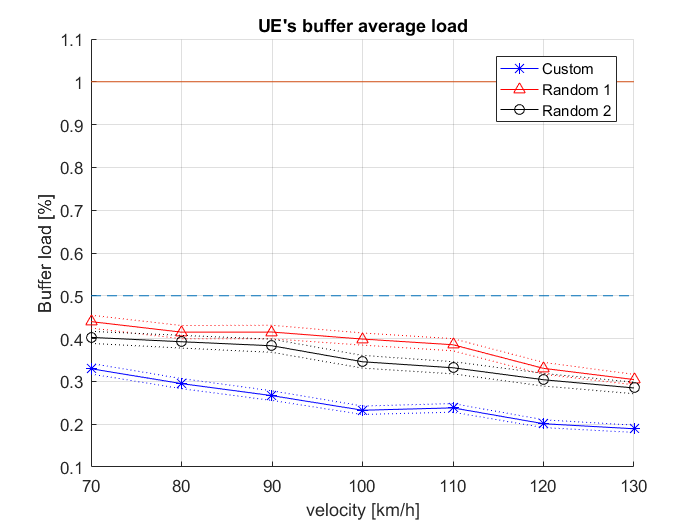
\includegraphics[width=9cm]{UE_buffer.png}
	\caption{Buffer load at UE side, for 14 BS per sector. Confidence intervals are at 95\%.}
	\label{fig:7BS_buffer_load}
\end{figure}

\begin{figure}[t]
	\centering
	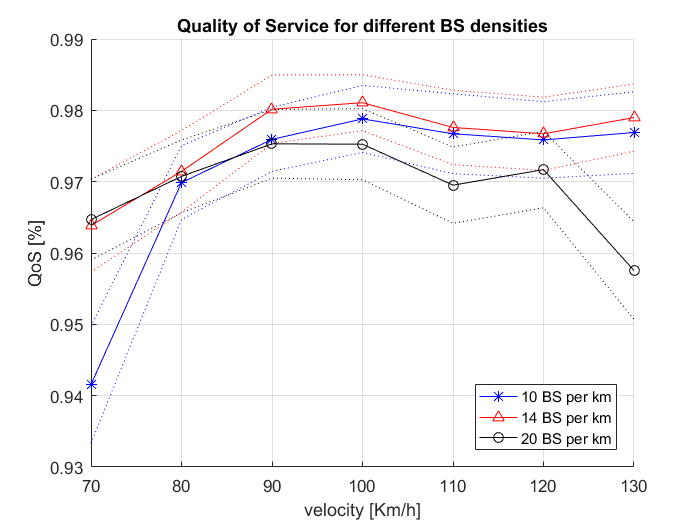
\includegraphics[width=9cm]{QoS_10-14-20-BS_densities.png}
	\caption{QoS for densities of 10, 14 and 20 BS per sector. Confidence intervals are at 95\%.}
	\label{fig:QoS_all}
\end{figure}

\begin{figure}[t]
	\centering
	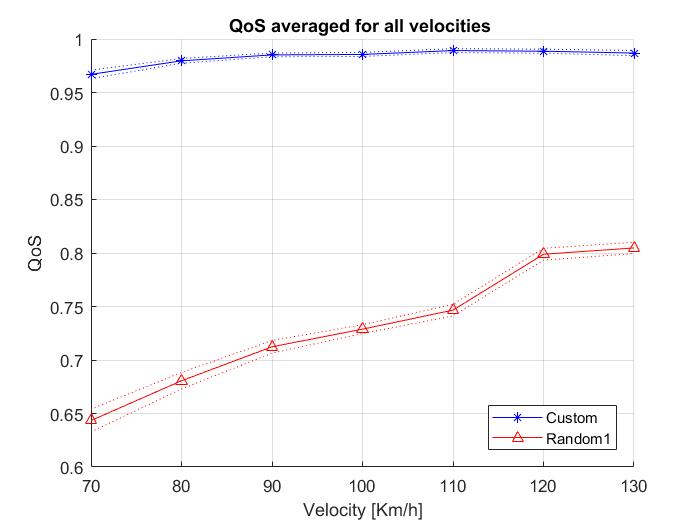
\includegraphics[width=0.5\textwidth]{QoS_20km.jpg}
	\caption{QoS for 20km long journey, 14 BS per sector. Confidence intervals are at 95\%.}
	\label{fig:QoS_20km}
\end{figure}

%%%%%%%%%%%%%%%%%%%%%%%%%%%%%%%%%%%
\section{Conclusions}\label{sec:conclusion}
%%%%%%%%%%%%%%%%%%%%%%%%%%%%%%%%%%%
Although our approach does not refer to sophisticated mathematical theories, it can attain high QoS for video streaming services in mobile scenarios. Obviously, to obtain optimal results, this system cannot work indipendently but has to be assisted, for instance, by another system that allows BSs to communicate to each other, in a way such that leftover data at BSs aren't lost but can be transferred from one BS to the other. In this way, UE could also transmit control informations about its buffer, in order to force BSs stopping the trasmission of new data when the buffer is full and redistribuiting the file along access points  to further minimize data loss.



\bibliographystyle{IEEEtran}
%standard bibliography
\begin{thebibliography}{10}
\bibitem[1]{}
J. G. Andrews et al., "What Will 5G Be?," in IEEE Journal on Selected Areas in Communications, vol. 32, no. 6, pp. 1065-1082, June 2014.

\bibitem[2]{}
T. Bai and R. W. Heath, "Coverage and Rate Analysis for Millimeter-Wave Cellular Networks," in IEEE Transactions on Wireless Communications, vol. 14, no. 2, pp. 1100-1114, Feb. 2015.

\bibitem[3]{}
Rappaport T.S., Sun S., Mayzus R., Zhao H., Azar Y., Wang K., Wong G.N., Schulz J.K., Samimi M., Gutierrez F., 2013, 'Millimeter wave mobile communications for 5G cellular: It will work!' IEEE Access, vol 1, pp. 335-349.

\bibitem[4]{}
H. Shokri-Ghadikolaei, C. Fischione, G. Fodor, P. Popovski and M. Zorzi, "Millimeter Wave Cellular Networks: A MAC Layer Perspective," in IEEE Transactions on Communications, vol. 63, no. 10, pp. 3437-3458, Oct. 2015.

\bibitem[5]{}
F. Boccardi, R. W. Heath, A. Lozano, T. L. Marzetta and P. Popovski, "Five disruptive technology directions for 5G," in IEEE Communications Magazine, vol. 52, no. 2, pp. 74-80, February 2014.

\bibitem[6]{}
G. Karagiannis et al., "Vehicular Networking: A Survey and Tutorial on Requirements, Architectures, Challenges, Standard and Solutions" in IEEE Communications Surveys and Tutorials, vol. 13, no. 4, pp. 584-616, Fourth Quarter 2011.

\bibitem[7]{}
M. Giordani, A. Zanella and M. Zorzi, "Millimeter wave communication in vehicular networks: Challenges and opportunities," 2017 6th International Conference on Modern Circuits and Systems Technologies (MOCAST), Thessaloniki, 2017, pp. 1-6.

\bibitem[8]{}
Prelcic, Nuria González et al. “Radar aided beam alignment in MmWave V2I communications supporting antenna diversity.” 2016 Information Theory and Applications Workshop (ITA) (2016): 1-7.

\bibitem[9]{}
J. Qiao, Y. He and X. S. Shen, "Proactive Caching for Mobile Video Streaming in Millimeter Wave 5G Networks," in IEEE Transactions on Wireless Communications, vol. 15, no. 10, pp. 7187-7198, Oct. 2016.

\bibitem[10]{}
E. Bastug, M. Bennis and M. Debbah, "Living on the edge: The role of proactive caching in 5G wireless networks," in IEEE Communications Magazine, vol. 52, no. 8, pp. 82-89, Aug. 2014.

\bibitem[11]{}
H. Ahlehagh and S. Dey, "Video caching in Radio Access Network: Impact on delay and capacity," 2012 IEEE Wireless Communications and Networking Conference (WCNC), Shanghai, 2012, pp. 2276-2281.

\bibitem[12]{}
A. Mishra, M. Shin and W. A. Arbaush, "Context caching using neighbor graphs for fast handoffs in a wireless network," IEEE INFOCOM 2004, 2004, pp. 361.


\end{thebibliography}

\end{document}
